De la misma manera en que definimos que un participante no conoce si su cap ni sus fichas disponibles, definimos que un jugador no conozca esencialmente los desafíos de los que formó parte.\\
Modelamos entonces una clase GestorDeDesafíos, cuyas instancias no sólo saben los desafíos de un participante, sino que también es se encargan de crear desafíos y de generar el contexto para que se simule un partido de un desafío. Es por esta razón que la clase Gestor de Desafíos usa a la clase Simulador y a la clase Logger.
A su vez, dado que debe indicar las estadísticas de los jugadores para la simuación, conoce al RegistroDeEstadísticas. Dado que debe validar que el participante puede apostar la cantidad de fichas indicadas y además debe actualizar las fichas disponibles de un participante, conoce al GestorDeFichas. Finalmente, como el cap de un participante se puede modificar por el resultado de un desafío, el GestorDeDesafíos conoce al GestorDeCap.\\

Un desafío está representado por la clase Desafío y está compuesto por una apuesta, un EstadoDeDesafío, un participante desafiante y un equipo desafiante.\\
La idea de que un desafío posea un estado representa el hecho de que un desafío puede estar abierto, esperando a ser ejecutado o terminado. Esto se modela a través de la jerarquía de clases EstadoDeDesafio.\\
Aprovechando la existencia de un estado, hicimos uso del patrón de diseño State, proveeyendo un protocolo en común entre un desafío y su estado. De esta forma, podemos modificar el comportamiento del desafío en runtime y, por ejemplo, modelar que no se puede simular un desafío abierto, ni se le puede pedir un resultado a un desafío en ejecución. El estado conoce al desafío al que conoce, de manera tal de poder enviarle el mensaje para cambiar de estado.\\
El estado EstadoDeDesafioAbierto, solo responde al mensaje incribirDesafiado(unParticipante, unEquipo), a partir del cual instancia el EstadoDeDesafioPorEjecutar como corresponde con los datos del desafiado y le envía el mensaje para cambiar de estado al desafío con el nuevo estado instanciado. Para todos lo demás mensajes lanza una excepción.
Análogamente, el EstadoDeDesafioPorEjecutar responder al mensaje realizarCon(unSimulador, unLogger) a partir del cual instancia un Partido y ejecuta la simulación. Finalmente, con los datos que poseía más el resultado del Partido, instancia un EstadoDeDesafioTerminado y le envía el mensaje de cambiar de estado al desafío a EstadoDeDesafioTerminado. Además responder a los mensajes desafiado() y equipoDesafiado(). Para todos los demás mensajes lanza una excepción.
Finalmente el EstadoDeDesafíoTerminado responde solamente a los mensajes ganador(), perdedor(), resultado(), desafiante(), equipoDesafiante() y para todos los demás mensajes lanza una excepción.

A través del GestorDeDesafíos se puede lanzar un desafío a través del mensaje incribirDesafío(unParticipante, unEquipo, unaApuesta). El GestorDeDesafíos, al recibir este mensaje, valida que la apuesta pueda realizarse para el participante y que el equipo pertenezca al participante desafiante. Luego, genera una nueva instancia de Desafío con el participante como desafiante, el equipo como equipo desafiante y la apuesta como la apuesta y con EstadoDeDesafíoAbierto.\\
Análogamente, mediante el mensaje aceptarDesafio(unParticipante, unEquipo, unDesafio) busca el desafío en cuestión, valida que el participante pueda realizar la apuesta y que el equipo perteneza al participante y luego le envía al desafío el mensaje incribirDesafiado(unParticipante, unEquipo) que lo reenviará a su estado.\\
Finalmente, mediante el la recepción del mensaje realizarDesafio(unDesafio), el GestorDeDesafios busca el desafío.Si lo encuenta, instancia un Simulador y un Logger y le envía al desafío el mensaje realizarCon(unSimulador, unLogger), que será reenviado a su estado.\\

El GestorDeDesafios además responde a los mensajes desafiosAbiertos(), desafiosFinalizados(), desafiosDe(unParticipante), desafiosAbiertosDe(unParticipante), desafiosGanadosPor(unParticipante), desafiosPerdidosPor(unParticipante), que no hacen más que filtrar los desafíos que se corresponden con los parámetros de búsqueda y los devuelve en una colección.\\

\begin{center}
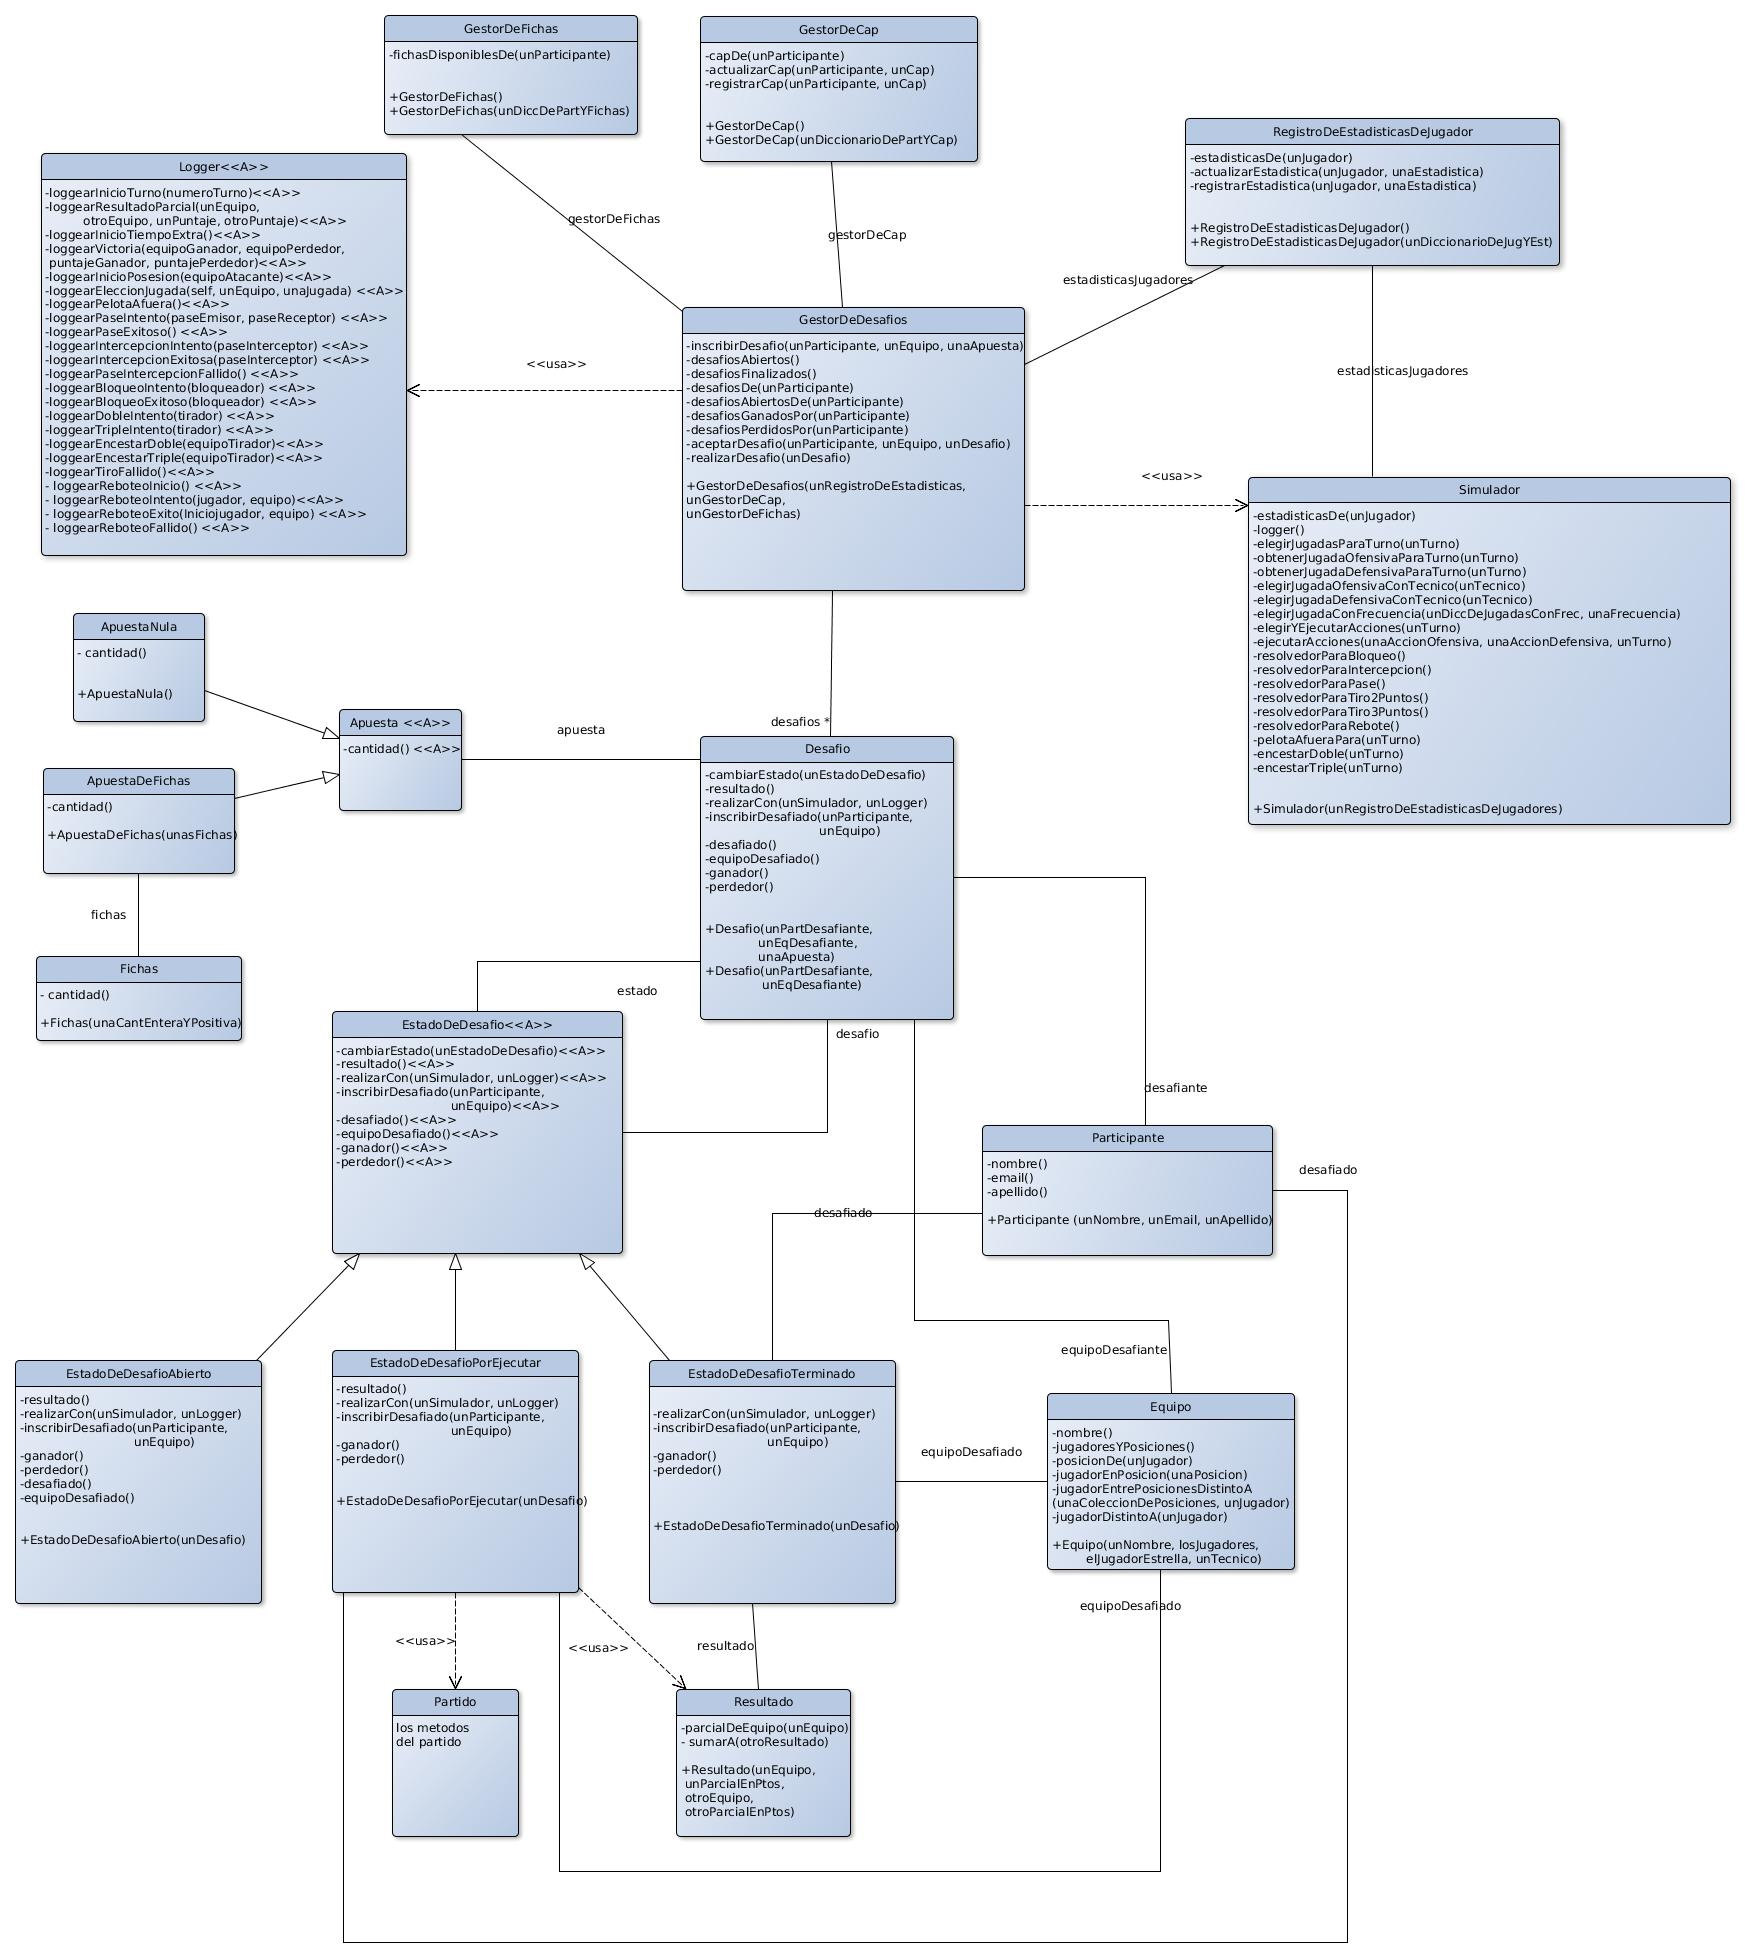
\includegraphics[scale=0.35]{diseno/gestionDeDesafios.jpg}
\end{center}